\section{Experiments}
\label{sec:exp}

The efficiency and scalability of Legion was examined by measuring the performance
of three applications on three clusters.  Table \ref{table:systems} summarizes 
the three clusters that were used.

\begin{tabular}{lccccc}
 & Nodes & CPUs/Node & GPUs/Node & DRAM/Node & Infiniband \\
sapling & 4 & 2x Xeon 5680 (HT enabled) & 2x Tesla C2070 & 48 GB & 2x QDR \\
viz & 10 & 2x Xeon 5680 (HT disabled) & 5x Quadro Q5000 & 24 GB & QDR \\
keeneland & 32* & 2x Xeon 5660 (HT disabled) & 3x Tesla M2090 & 24 GB & QDR 
\end{tabular}

Nodes with multiple instances of multiple resources are a challenge for 
existing programming models that have a flat model of the system (e.g. MPI).
They are faced with a choice of lumping all 
the resources together and ignoring the internal irregularities (e.g. NUMA
in multi-socket x86 systems) or of separating a single physical node into
multiple smaller nodes, ignoring the better affinity between sockets/GPUs/etc
on the same node and either wasting or over-subscribing some resources when
the quantities of different resources don't share a common divisor.

In contrast, the machine model used by the Legion runtime is based on an
affinity graph of CPUs and GPUs and is able to accurately capture complex
machine hierarchies.

For each application, multiple problem sizes were used, and each size problem was
run on subsets of each machine ranging from the smallest (a single CPU core or GPU)
to the largest or near-largest.  (Keeneland was an exception here - although it has
115 nodes, we limited our runs to at most 32 nodes to get sufficient cluster time.)
By looking at the performance of the same size problem over progressively larger
machines, we are able to measure the ``strong scaling'' that Legion is able to
achive.  By increasing the problem size as well, we also measure ``weak scaling''.

\subsection{Circuit Simulation}
\label{subsec:exp_ckt}

The first experiment run was the distributed circuit simulation, described in 
section \ref{sec:ex}, with all application code running on the CUDA-capable GPUs in
each node.  The application kernels are written in CUDA, while the Legion runtime
handles all the resource allocation, scheduling, and data movement.  In particular,
Legion's ability to efficiently manage, access, and move the irregularly partitioned
shared data around the system while keeping the private nodes and wires resident in
each GPU's framebuffer memory is critical in keeping the overhead low, a neccessity
for good scalability.

Circuits of two different sizes were simulated.  The first had 480K wires, connecting
120K nodes.  The second is twice as large, with nearly a million wires connecting a
quarter of a million nodes.  In addition to running these tests on varying number of
nodes, the number of GPUs used by the runtime was also varied.  In no case did the 
changes to nodes or number of GPUs per node require any changes to the application code.

The circuit simulation used a simple, but application-specific, mapper.  At initialization
time, the mapper queries the list of GPUs in the machine and identifies each GPU's
framebuffer memory and ``zero-copy'' memory (i.e. the pinned memory that both the GPU and
CPUs in the system can access directly).  Once the circuit is partitioned, the partitions
are assigned a ``home'' GPU in round-robin fashion.  Every task related to that partition is
then sent to that GPU, with no task stealing allowed.  (If the circuit is partitioned well,
there should be minimal load imbalance between the pieces, and the rebalancing benefit of 
moving a partition is unlikely to be worth the cost of moving all the 
private data for a piece from one GPU to another.)  The regions for a task are mapped as 
shown in figure \ref{fig:gpumapping}.

Figure \ref{fig:ckt_speed} shows the performance of the Legion circuit simulation relative
to a single-GPU implmementation hand-coded in CUDA.  Each line shows the scaling of
a particular problem size as the number of nodes is varied.  Our results demonstrate
excellent strong scaling behavior, with speedups of *??*x (compared to the single-GPU CUDA
version) for the small problem on 48 GPUs and *??*x for the larger problem size on 96 GPUs.

Figure \ref{fig:ckt_overhead} shows the fraction of the overall simulation time (summed over
all nodes) spent in the application kernels compared to the various pieces of the Legion
runtime.  As the node count increases, the non-communication overhead stays relatively constant.
Only the communication overhead grows, and it grows nearly linearly with the node count.
A linear growth in communication cost as a simulation is split over multiple nodes is to
be expected.

\begin{figure}
\subfigure[Circuit Simulation Speed Relative to Single-GPU Implementation]
{
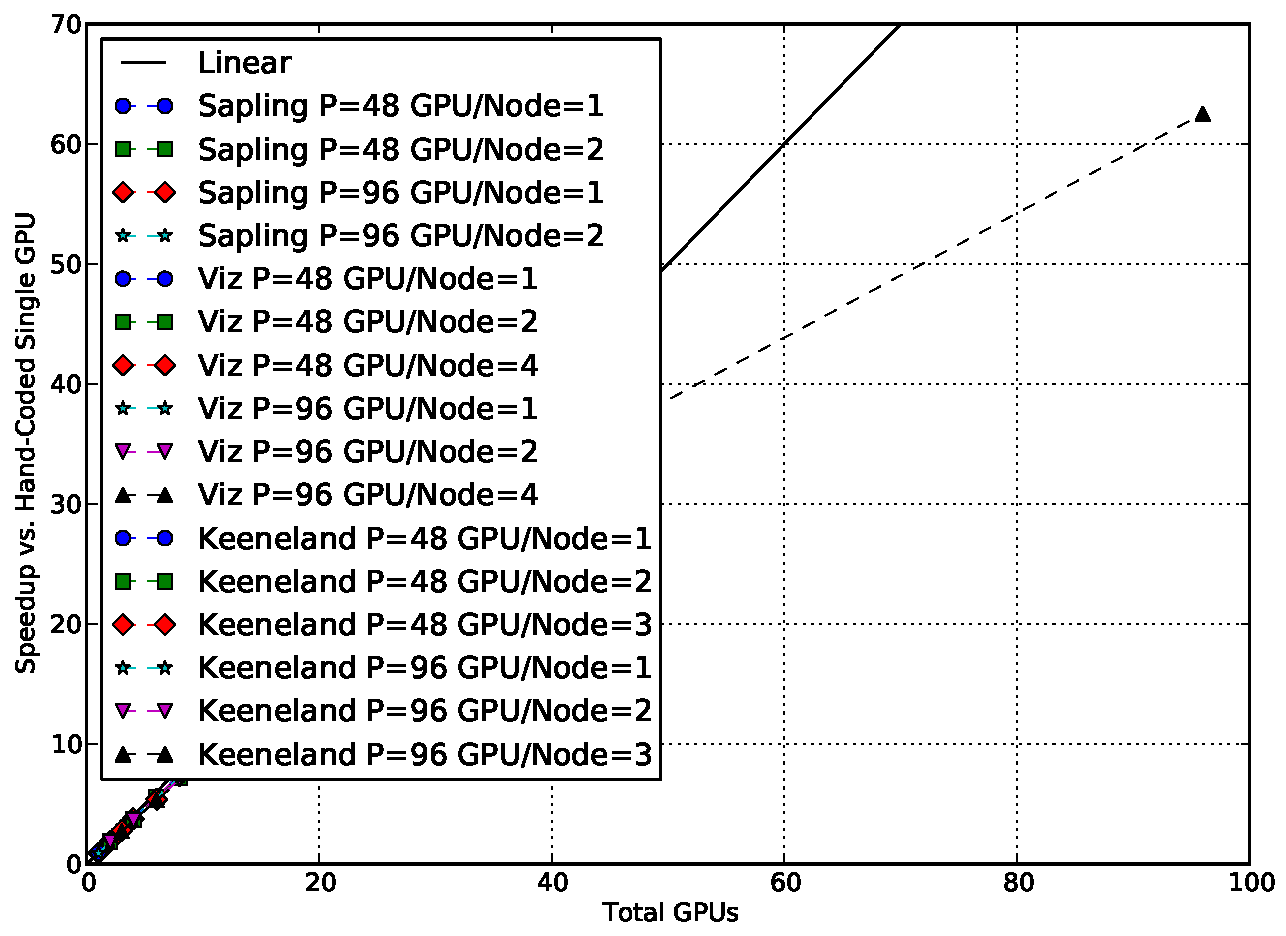
\includegraphics[scale=0.4]{figs/circuit_speedups.pdf}
\label{fig:ckt_speed}
}

\subfigure[Overhead of Circuit Simulation on Keeneland with 3 GPUs/Node]
{
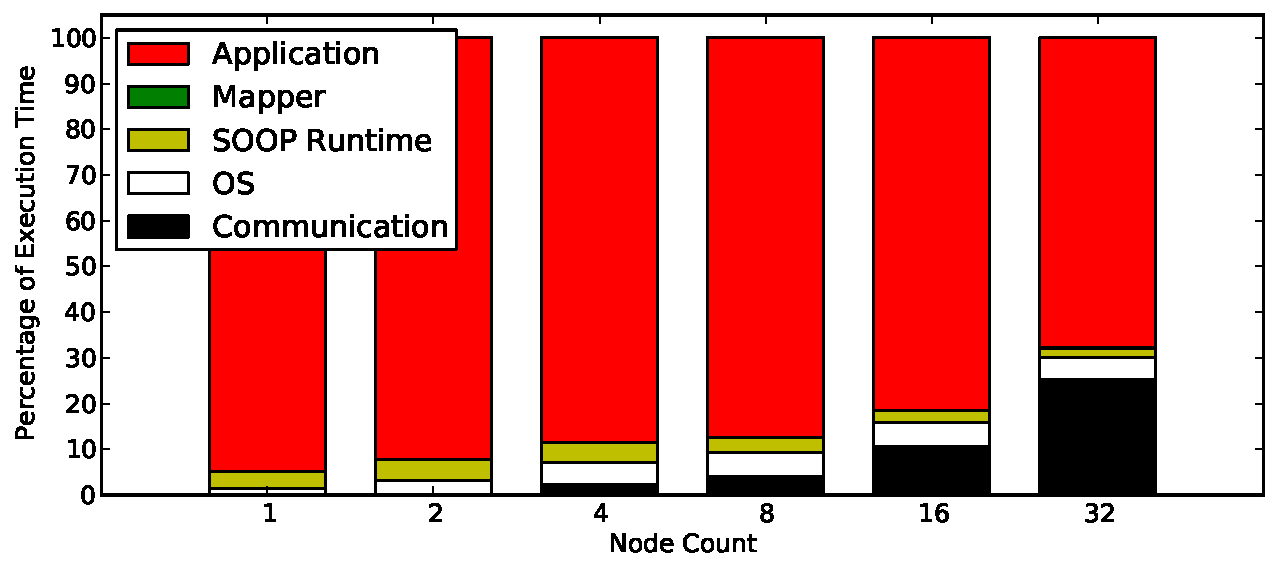
\includegraphics[scale=0.4]{figs/circuit_overhead.pdf}
\label{fig:ckt_overhead}
}
\caption{Circuit Simulation Results}
\end{figure}

\subsection{Particle Simulation}
\label{subsec:exp_fluid}

Our second experiment is a port of the \emph{fluidanimate} benchmark from the PARSEC suite\cite{bienia11benchmarking},
which does a particle-based simulation of a fluid.  Each particle interacts only with other nearby
particles, so the benchmark divides the space in which the fluid
can move into a three-dimensional array of cells such that the range of interaction is limited to just the
cells adjacent (including diagonals) to the one a particle resides in.  Originally designed to be a
chip multiprocessor benchmark, the application divides the array into ``grids'' and assigns each one to 
a thread.  Per particle locking is used to safely access particles in cells that lie
on the edge of a grid.  This fine-grained locking along with the assumption of a shared address space lead to
good scaling in a multi-core processor, but rule out any attempt to scale beyond a single node.  To extend the
scaling further, our port divides uses region partitioning to divide the array into grids in a similar
way, but handles the interaction between grids in a way that doesn't rely on access to uniform shared memory.
Instead, the Legion version of the benchmark creates explicit ghost copies of cells on the boundaries of grids
and uses those ghost cells to exchange information between the grids.

The mapper for the particle simulation is very simple - it just maps one grid's tasks onto each processor and
maps all regions for that grid (both the internal the ghost cells) into the system memory used by that processor.
The exchange of the ghost cell data between processors is handled by the Legion runtime as a ghost cell region
gets alternately mapped in two different memories.

Figure \ref{fig:fluid_single} compares the performance of the Legion implementation against the PARSEC version,
using a relatively small problem (300K particles on a 15x21x15 array of cells).  Between 1 and 4 threads, the
results for sapling are nearly indistinguishable, indicating 
neither the Legion runtime nor the the restructuring of the implementation to allow multi-node scaling impose
any significant overhead.  In fact, it's possible that the use of explicit ghost cells rather than 
fine-grained sharing of cache lines might be a net win.  At 8 threads and above, the performance begins to vary.
Both the Legion and PARSEC version on viz flatten out as they over-subscribe the 12 physical cores.  On sapling,
which has HyperThreading enabled, deviations from linear begin sooner as the operating system's scheduler's
thread placement choices begin to matter.

To measure scaling beyond a single node, three different problem sizes were run for each of the three systems,
 with the results plotted in figure
\ref{fig:fluid_multi}.  For the smallest problem (300K particles), we observe a 20\% speedup when going to 1
node to 2 (a total of 16 threads), but begin slowing down beyond that due to communication overhead - at 4 nodes
there are twice as many ghost cells as interior grid cells.  The larger problem sizes (2.4M and 19M
particles) do much better, with scaling of up to 5.4x when going from 1 node up to 16.

%Although the particle simulation being performed is on a regular array of cells, it turns out that the
%distribution of particles amongst the cells is very irregular.  The simulation models gravity, which points in
%the -Y direction, so the particles are clustered mostly in the lower half of the cell array.  The PARSEC
%implementation works around this imbalance by only slicing the cell array through the X and Z axes, yielding
%grids that are uniformly populated, even if the number of boundary cells (for which locks must be used) is
%increased above the minimum. MORE TEXT NEEDED HERE

\begin{figure}
\subfigure[Single-Node Particle Simulation Speed]
{
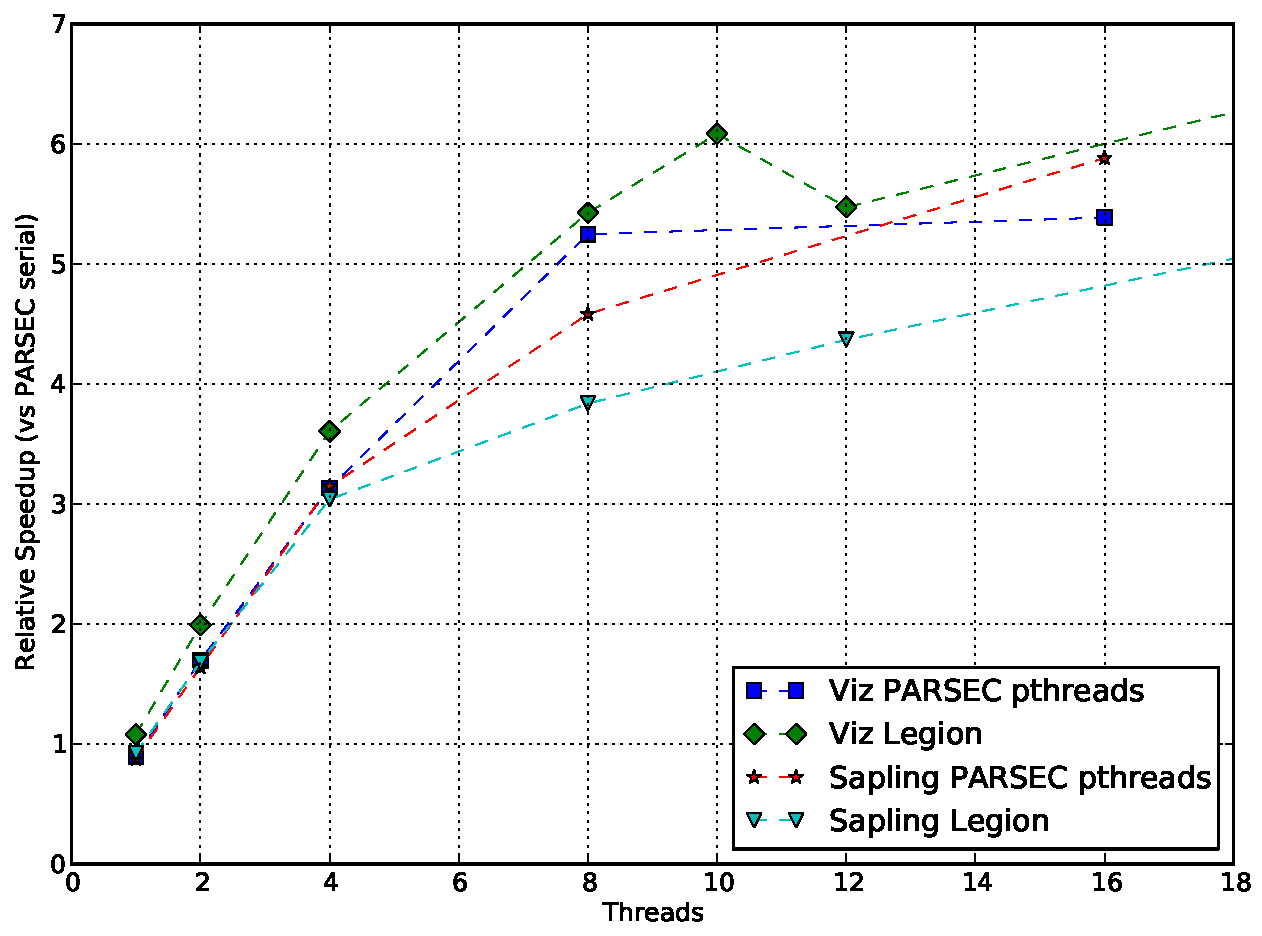
\includegraphics[scale=0.4]{figs/fluid_singlenode.pdf}
\label{fig:fluid_single}
}

\subfigure[Multi-Node Scaling]
{
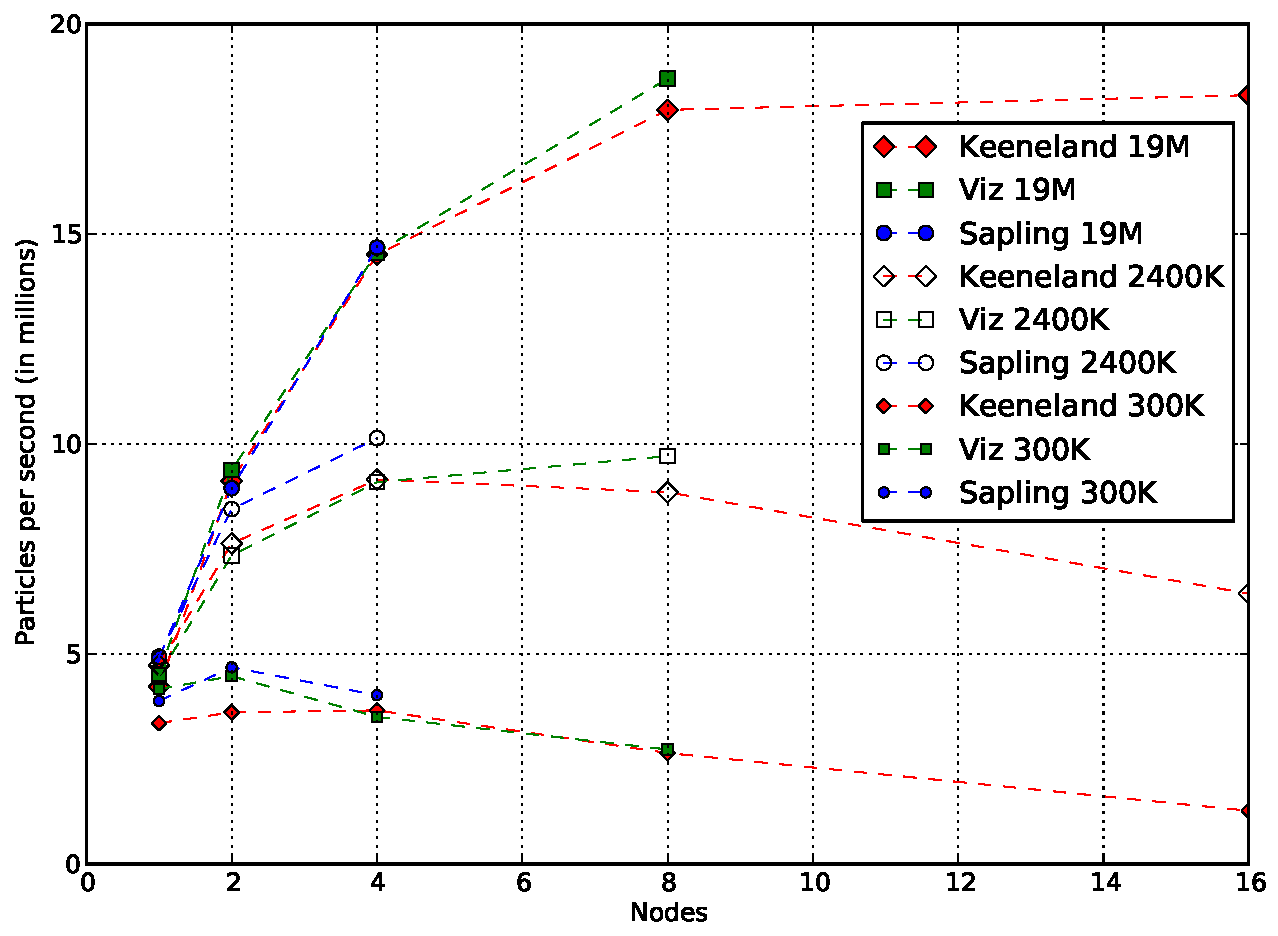
\includegraphics[scale=0.4]{figs/fluid_multinode.pdf}
\label{fig:fluid_multi}
}

%\subfigure[Effect of Load-Balanced Partitioning]
%{
%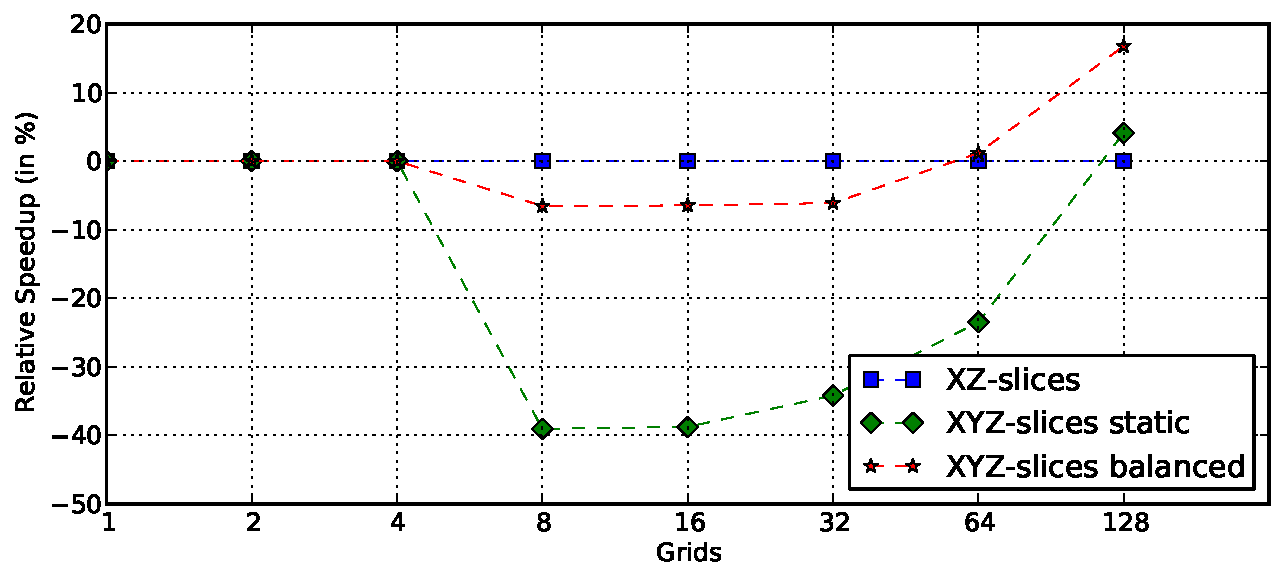
\includegraphics[scale=0.4]{figs/fluid_balance.pdf}
%\label{fig:fluid_balance}
%}
\caption{Fluid Simulation Results}
\end{figure}

\subsection{Adaptive Mesh Refinement}
\label{subsec:exp_amr}

\begin{figure}
\subfigure[Sapling Results]
{
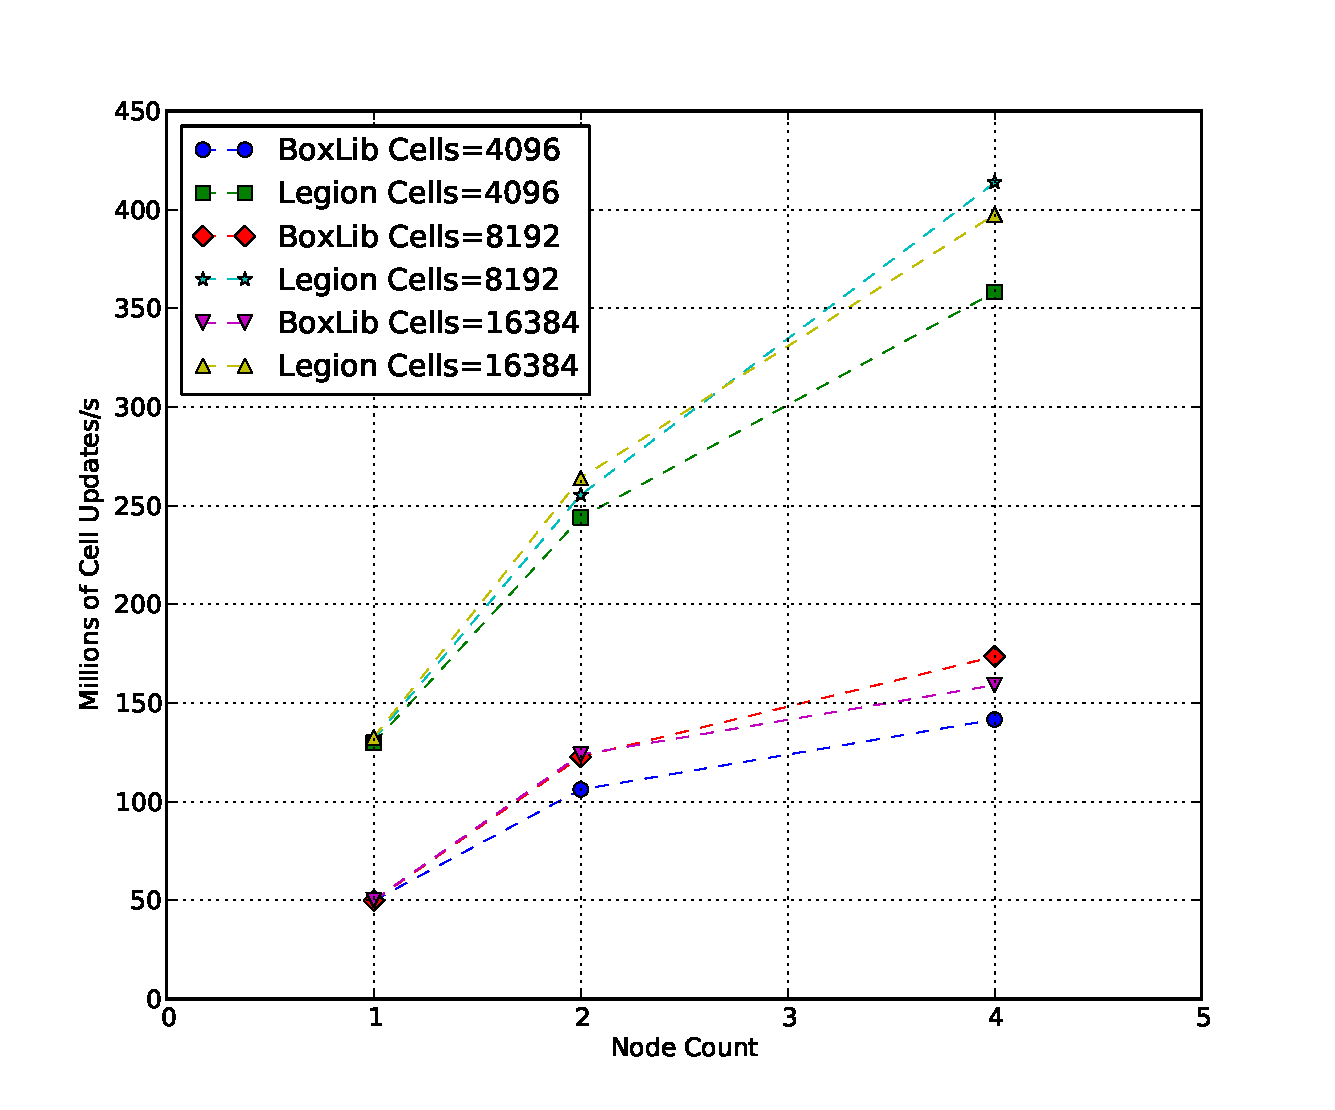
\includegraphics[scale=0.4]{figs/Sapling_amr.pdf}
\label{fig:amr_sapling}
}

\subfigure[Viz Results]
{
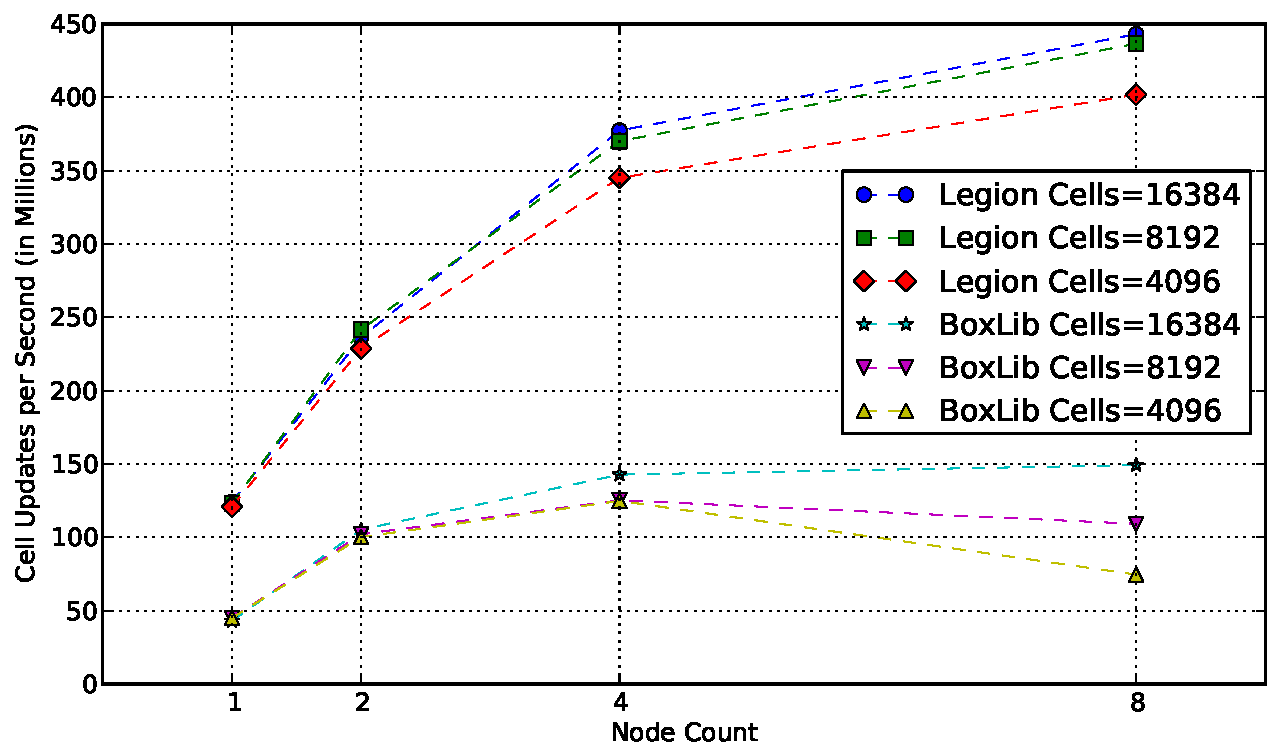
\includegraphics[scale=0.4]{figs/Viz_amr.pdf}
\label{fig:amr_viz}
}

\subfigure[Keeneland Results]
{
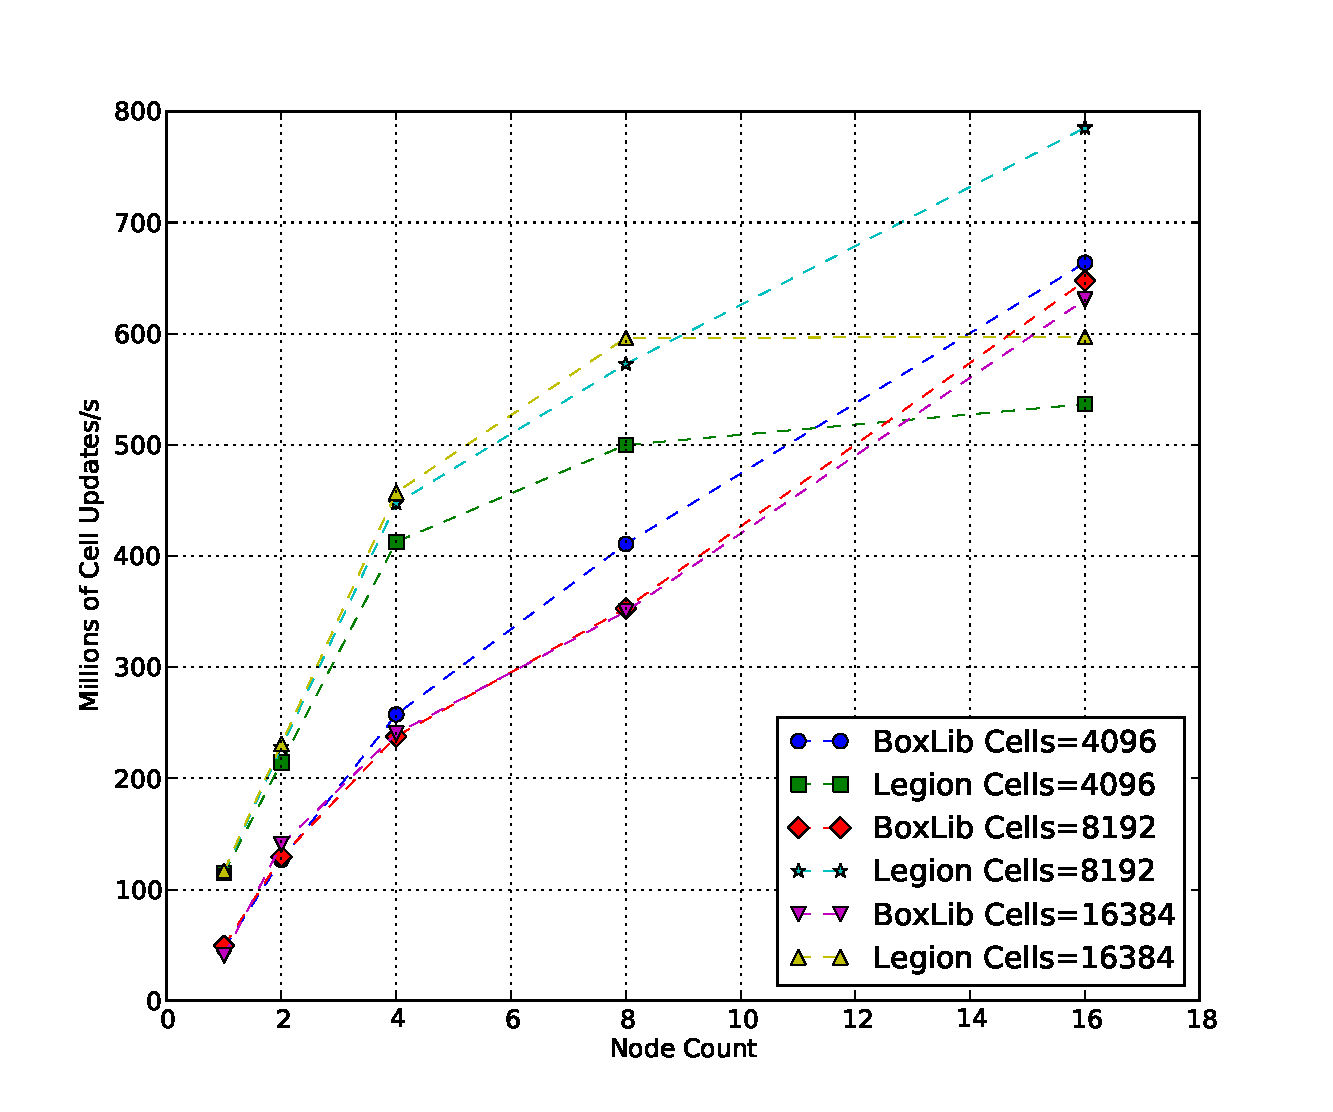
\includegraphics[scale=0.4]{figs/Keeneland_amr.pdf}
\label{fig:amr_keeneland}
}
\caption{Adaptive Mesh Refinement Results}
\end{figure}
